\documentclass[tikz,border=5mm]{standalone}
\usepackage{tikz}
\usetikzlibrary{shapes.geometric, shapes.multipart, arrows.meta, positioning, calc, fit, backgrounds, shadows, decorations.pathreplacing, matrix, patterns}

\begin{document}
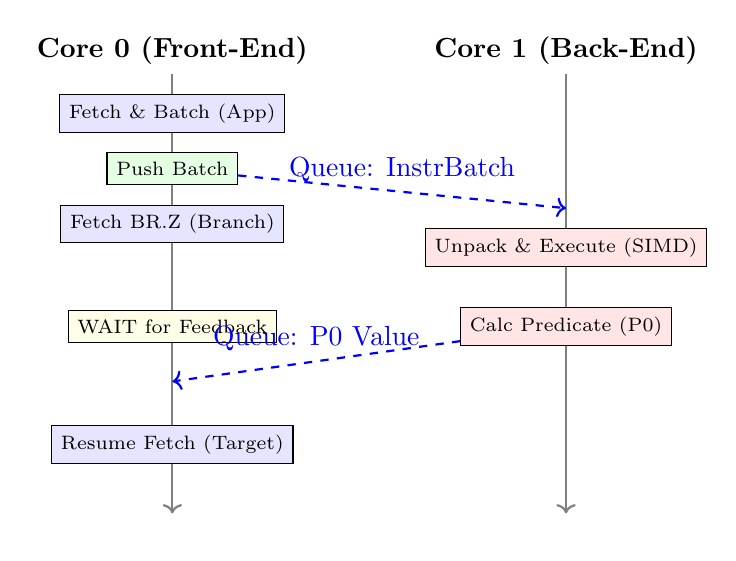
\begin{tikzpicture}[node distance=2cm, auto,
    timeline/.style={->, thick, gray},
    msg/.style={->, thick, blue, dashed},
    box/.style={rectangle, draw, fill=white, font=\scriptsize}]

    % Timelines
    \node (c0_top) at (0,0) {\textbf{Core 0 (Front-End)}};
    \node (c1_top) at (5,0) {\textbf{Core 1 (Back-End)}};
    \node (c0_bot) at (0,-6) {};
    \node (c1_bot) at (5,-6) {};

    \draw[timeline] (c0_top) -- (c0_bot);
    \draw[timeline] (c1_top) -- (c1_bot);

    % Sequence Steps
    
    % 1. Fetch
    \node[box, fill=blue!10] (f1) at (0, -0.8) {Fetch \& Batch (App)};
    
    % 2. Push Batch
    \node[box, fill=green!10] (push1) at (0, -1.5) {Push Batch};
    \draw[msg] (push1) -- node[above] {Queue: InstrBatch} (5, -2.0);
    
    % 3. C1 Execute
    \node[box, fill=red!10] (exec1) at (5, -2.5) {Unpack \& Execute (SIMD)};
    
    % 4. C0 continues fetching (Run Ahead)
    \node[box, fill=blue!10] (f2) at (0, -2.2) {Fetch BR.Z (Branch)};
    
    % 5. C0 waits for feedback
    \node[box, fill=yellow!10] (wait) at (0, -3.5) {WAIT for Feedback};
    
    % 6. C1 processes branch dependency
    \node[box, fill=red!10] (exec2) at (5, -3.5) {Calc Predicate (P0)};
    
    % 7. Feedback
    \draw[msg] (exec2) -- node[above] {Queue: P0 Value} (0, -4.2);
    
    % 8. Resume
    \node[box, fill=blue!10] (resume) at (0, -5.0) {Resume Fetch (Target)};

\end{tikzpicture}
\end{document}
